\chapter{Travail d'analyse}
	
	\section*{Introduction}
	
	Le but de notre projet est de reconstruire la vue aérienne d'un glacier
	à partir de photos au sol et de points de contrôle (points sur une image
	dont on connait la latitude et la longitude).	
	
	Nous allons décrire les besoins du projets, les outils que 
	nous avons sélectionnés pour le bon déroulement du projet et
	enfin le résultat de nos recherches sur les algorithmes que
	nous allons implémenter pour répondre aux besoins.
	 
	\section{Gestion du projet}
	
	Afin d'organiser au mieux le projet, nous allons définir les besoins
	et mettre en place des outils de gestion de projet.
	
		\subsection{Analyse des besoins}
		
	Les besoins du projet sont les suivants:
		
	\begin{itemize}
		\item Lire et écrire une image
		\item Déterminer la longitude et la latitude d'un point d'une image
		\item Reporter une image sur la vue aérienne à construire
	\end{itemize}
		
	~
		
	Nous disposons de plusieurs images dont on connait la latitude et la
	longitude de certains points. La problématique du projet
	est que le relief de l'image n'est pas régulié, par conséquent une
	méthode classique telle que la méthode des moindres carrés~\cite{carre} 
	ne peut pas être appliquée.
		
	Les algorithmes mis en place pour résoudre cette problématique sont
	décrits dans la section \ref{section:recherche}.
		
		\subsection{Outils de gestion de projet}
		
	Nous allons maintenant décrire les outils mis en place au bon
	déroulement du projet.
	
		\paragraph{Gantt} 
		
	Afin de gérer au mieux l'organisation temporelle du projet, nous avons
	créer un diagramme de Gantt, voir figure \ref{figure:gantt}.
	
	\begin{figure}[ht]
	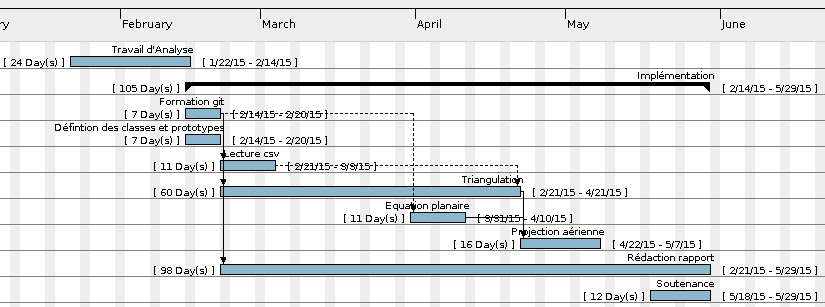
\includegraphics[max size={\textwidth}{\textheight}]{contents/img/gantt.png}
	\caption{Diagramme de Gantt}
	\label{figure:gantt}
	\end{figure}
		
		\paragraph{Gitlab} 
		
	Afin de partager de la manière la plus efficace possible notre code
	source, nous allons utiliser le logiciel \textit{git} et la plateforme
	gitlab de l'EISTI. Cependant, un seul membre du groupe est formé à ce
	logiciel, par conséquent, une formation préalable est nécessaire.
	

		\paragraph{Jenkins et SonarQube}
		
	Jenkins et SonarQube sont des outils permettant respectivement
	l'intégration continue et l'évaluation de la qualité du code.
	Cependant, du fait qu'une partie de l'équipe ne maitrise pas git, nous
	avons décidé de ne pas mettre en place Jenkins et SonarQube immédiatement
	afin de pouvoir nous concentrer sur les algorithmes à mettre en place et
	l'apprentissage de git.

	\begin{figure}[ht]
	\centering
	
\includegraphics[scale=0.5]{contents/img/logos.png}
	\caption{Logo de gitlab, jenkins et SonarQube}
	\end{figure}
			
	\section{Résultats de nos recherches}
		\label{section:recherche}
		
	Nous allons maintenant décrire les résultats de nos recherches et les
	algorithmes complexes que nous allons implémenter.	
			
		\subsection{\'Etat de l'art}
		
	Nous avons au préalable fait un état de l'art. Nous avons trouvé un
	article scientifique~\cite{bernard} présentant exactement notre problème.
	Dans cet article, les  auteurs décrivent comment ils ont reconstruit une
	image aérienne à partir d'images enregistrées par des caméras. De plus,
	ces derniers ont également réussi à corriger le dérèglement des caméras dû
	aux conditions météorologiques au fil des jours (nous ne traitons pas cette
	partie). 
	
	Leur succès nous garantit que leur méthode est efficace.
			
		\subsection{Triangulation de Delaunay}
		
	Nous avons donc choisi d'implémenter une triangulation de Delaunay. Nous 
	avons trouvé 2 algorithmes~\cite{delaunay} pour la triangulation de
	Delaunay, une récursive, une itérative. Le premier est en
	$\Omega(n\log n)$ et le second est en $O(n^2)$. L'avantage du second est
	qu'il est plus simple et plus facile à implémenter. De plus, comme
	dans notre application $n_{max} = 640$ un algorithme en $O(n^2)$ reste
	envisageable. Nous avons cependant choisi d'implémenter le 1er, par soucis
	de performance.
	
	~	
	
	L'algorithme récursive repose sur une approche \textit{divide and conquer}.
	En effet, il sépare l'ensemble de points en deux, calcule la triangulation
	des deux ensembles et les fusionne. La principale difficulté est le calcul
	récursif simultané de l'enveloppe convexe~\cite{convexe} ainsi que du
	\textit{backtracking} de données, comme par exemple le point le plus à
	gauche de l'enveloppe convexe.
	
	Il n'est pas pertinent d'écrire ici le pseudo code des
	algorithmes, car ils sont disponibles dans notre bibliographie.
	
	~	
	
	En revanche, nous allons décrire ce que permet l'algorithme et pourquoi
	nous l'utilisons. L'algorithme permet à partir d'un ensemble de point $P$,
	qui sont nos points de contrôles, de former une triangulation $DT(P)$ tels
	qu'aucun des points $P$ n'est à l'intérieur du cercle circonscrit d'un des
	triangles de $DT(P)$. Voir figure \ref{figure:triangles}.
			
	\begin{figure}[!h]
	\centering
	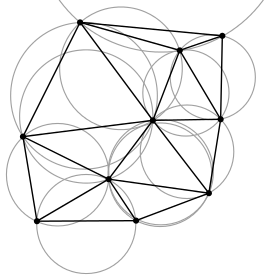
\includegraphics[scale=0.6]{contents/img/triangles.png}
	\caption{Une triangulation de Delaunay}
	\label{figure:triangles}
	\end{figure}
		
	Appliqué à notre problème, l'algorithme donne le résultat suivant:~nous
	pouvons voir les points de contrôle sur la figure \ref{figure:controles} et
	le résultat de l'algorithme sur la figure \ref{figure:triangulation}.
	
	\begin{figure}[!ht]
	\centering
	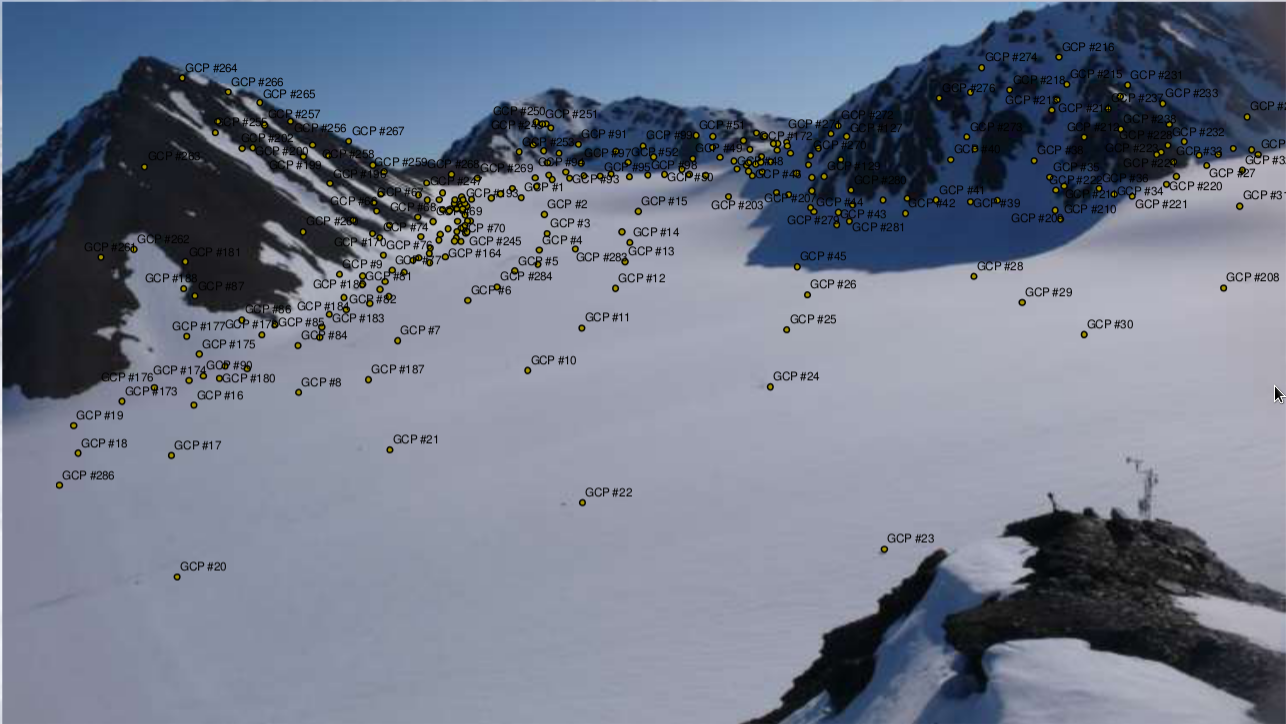
\includegraphics[max size={\textwidth}{\textheight}]{contents/img/controles.png}
	\caption{Les points de contr\^oles sur une image}
	\label{figure:controles}
	\end{figure}
	
	\begin{figure}[!hb]
	\centering
	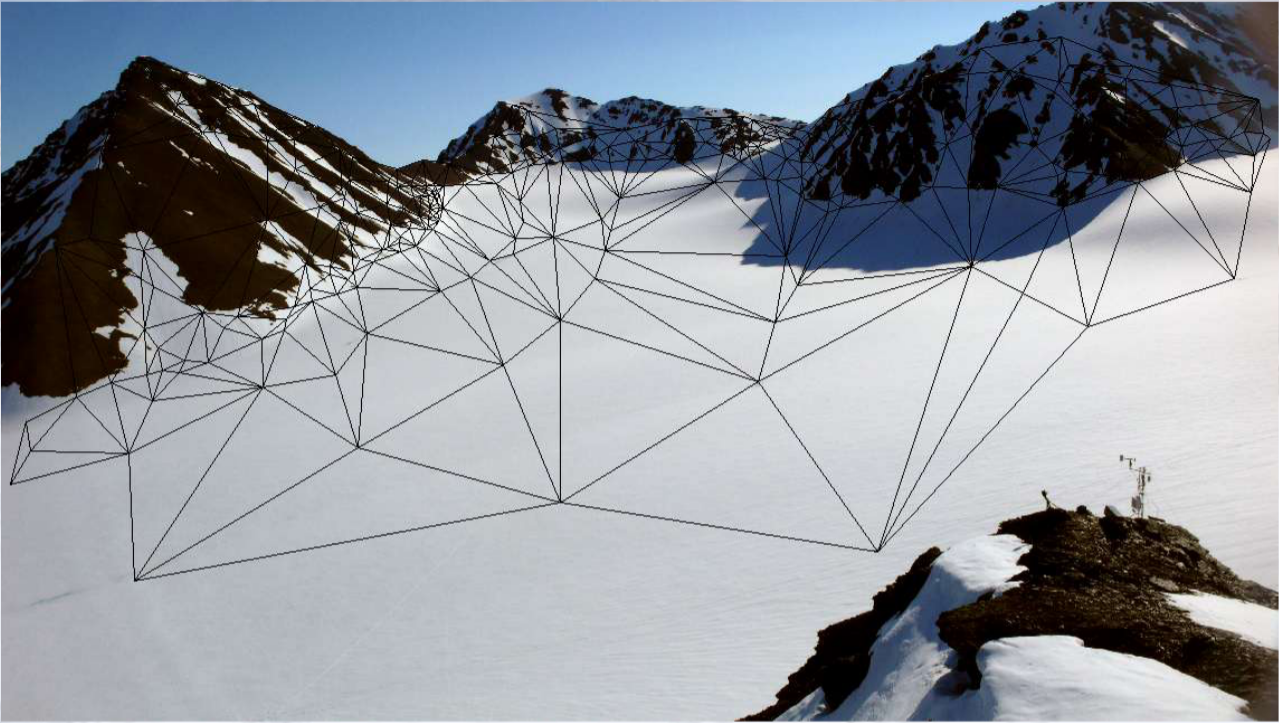
\includegraphics[max size={\textwidth}{\textheight}]{contents/img/triangulation.png}
	\caption{Triangulation de Delaunay appliquée à notre image}
	\label{figure:triangulation}
	\end{figure}
	
	Nous pouvons remarquer qu'à l'intérieur d'un triangle, le relief est
	relativement régulié. C'est pourquoi, connaissant la latitude et la
	longitude des 3 points qui forment le triangle, nous pouvons approximer
	la latitude et la longitude des points à l'intérieur du triangle. Cette
	méthode est décrite dans la sous partie suivante \ref{subsection:plan}. 
	
	Plus de détails sur les structures de données utilisées seront décrites 
	lors de l'implémentation.
			
		\subsection{Résolution d'équation planaire}
			\label{subsection:plan}
		
	A l'intérieur d'un triangle, nous supposons que la lattitude et la 
	longitude varient de façon linéaire par rapport aux coordonnées x et y.
	De ce fait nous cherchons deux équations planaires :
	
	\begin{equation}
	\left\{
		\begin{array}{l}
			L = ax + by + c\\ 
  			H = a'x + b'y + c'
		\end{array}
	\right.
	\end{equation}
	
	Nous disposons des 3 points du triangle qui sont des points de contr\^ole,
	nous pouvons donc parfaitement déterminer les inconnus $a, b, c, a', b'$
	et $c'$ (pivot de Gauss~\cite{gauss}). Il suffit donc de faire cela pour 
	tous les triangles pour conna\^itre la lattitude et la longitude de chaque
	point de l'image.
	
	Nous sommes alors capable de réaliser la projection de la latitude et 
	longitude sur notre image (voir figure \ref{figure:projection}). On peut 
	alors reporter l'image sur la vue aérienne.
	
	\begin{figure}[!ht]
	\centering
	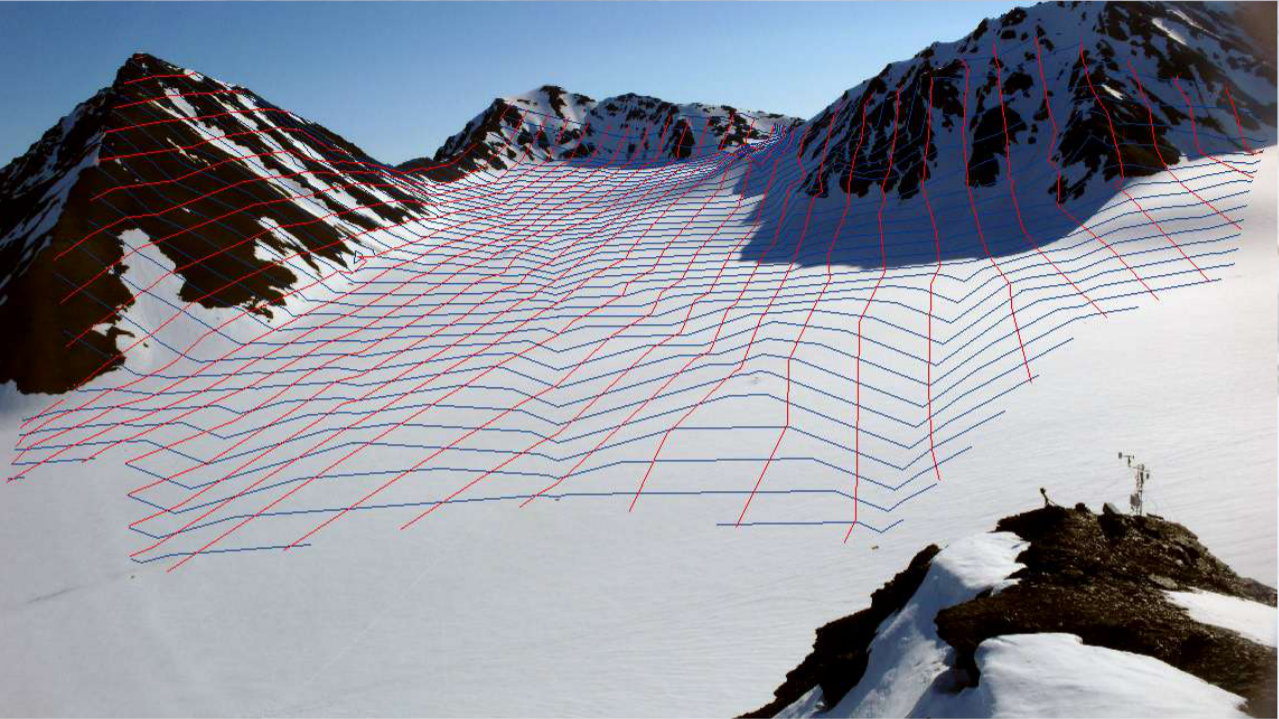
\includegraphics[max size={\textwidth}{\textheight}]{contents/img/projection.png}
	\caption{Projection de la latitude et de la longitude sur l'image}
	\label{figure:projection}
	\end{figure}

	\section*{Conclusion}
	
	Finalement, nous savons quels algorithmes utiliser pour créer une image
	aérienne du glacier. Nous avons réparti notre travail dans le temps. 
	
	Nous pouvons donc passer à l'étape suivante, c'est à dire, 
	l'implémentation.
	